\documentclass[final, 12pt]{beamer}
\usepackage[utf8]{inputenc}
\usepackage[orientation=portrait, size=a0, scale=1.5]{beamerposter}
\usenavigationsymbolstemplate{\beamertemplatenavigationsymbolsempty}

\usepackage{ragged2e}
\usepackage{graphicx}
\usepackage{tikz}
\usetikzlibrary{positioning}

% set widths
\newlength{\colwidth}
\setlength{\colwidth}{0.435\paperwidth}

% fonts
\setbeamercolor{block title}{fg=violet,bg=white}
\setbeamercolor{block body}{fg=black,bg=white}
\setbeamercolor{item}{fg=black}
\setbeamerfont{caption}{size=\normalsize, series=\bfseries}
\setbeamerfont{block title}{series=\bfseries}
\renewcommand{\figurename}{\color{black}{Figure}}

% maths
\newcommand{\vt}[2][t]{\nu_{#1}^{(#2)}}
\newcommand{\E}{\mathbb{E}}

% block style
\setbeamertemplate{block begin}
{
  \par\vskip\medskipamount
  \vskip0.8cm
  \begin{beamercolorbox}[colsep*=0.5ex,dp={2ex},center]{block title}
     \vskip-1cm
    \usebeamerfont{block title}\Large\insertblocktitle
  \end{beamercolorbox}
  {\parskip0pt\par}
  \ifbeamercolorempty[bg]{block title}
  {}
  {\ifbeamercolorempty[bg]{block body}{}{\nointerlineskip\vskip-0.5pt}}
  \vskip0.5cm
  \usebeamerfont{block body}
  \vskip-0.5cm
  \begin{beamercolorbox}[colsep*=0ex,vmode]{block body}
}
\setbeamertemplate{block end}
{
  \end{beamercolorbox}
  \vskip\smallskipamount
}

% title section
\title{Genealogies of Sequential Monte Carlo Algorithms}
\author{Suzie Brown}
\institute{Department of Statistics, University of Warwick}
%\logo{
\includegraphics[scale=1.8]{../oxwasp3.png}}
\date{}


\begin{document}
\begin{frame}

\vspace*{-20pt}

\centering
\makebox[\textwidth]{
\includegraphics[width=\paperwidth]{../warwickhead.png}}

\vspace*{-360pt}

\huge{\inserttitle}\\[2pt]
\LARGE{\insertauthor}\\[7pt]
\large{with Paul Jenkins, Adam Johansen and Jere Koskela}\\[7pt]
\normalsize{\insertinstitute}\\[5pt]
\normalsize{S.Brown.18@warwick.ac.uk}\\[25pt]

\vspace*{5pt}

\hrule

\vspace*{-10pt}

\begin{columns}
\begin{column}{\colwidth}
\begin{block}{Sequential Monte Carlo}

SMC\textsuperscript{1} is an effective Monte Carlo method for models with strong correlation between parameters. For example, inferring a sequence of underlying parameters from an autocorrelated time series.\\[16pt]

We approximate distributions by samples of ``particles''. The algorithm starts with $N$ equally-weighted particles and repeats the steps:
\begin{center}
\resizebox{0.85\colwidth}{!}{%
\begin{tikzpicture}
\filldraw[violet] (0,0) circle (6pt);
\filldraw[violet] (0,1) circle (6pt);
\filldraw[violet] (0,1.5) circle (6pt);
\filldraw[violet] (0,2.2) circle (6pt);

\draw[->] (0.4,2.2) -- (4.6,3);
\draw[->] (0.4,1.5) -- (4.6,1.2);
\draw[->] (0.4,1) -- (4.6,-0.9);
\draw[->] (0.4,0) -- (4.6,0.3);

\filldraw[violet] (5,0.3) circle (6pt);
\filldraw[violet] (5,-0.9) circle (6pt);
\filldraw[violet] (5,1.2) circle (6pt);
\filldraw[violet] (5,3) circle (6pt);

\draw[->] (5.5,3) -- (9.5,3);
\draw[->] (5.5,1.2) -- (9.5,1.2);
\draw[->] (5.5,-0.9) -- (9.5,-0.9);
\draw[->] (5.5,0.3) -- (9.5,0.3);

\filldraw[violet] (10,0.3) circle (11pt);
\filldraw[violet] (10,-0.9) circle (4pt);
\filldraw[violet] (10,1.2) circle (7pt);
\filldraw[violet] (10,3) circle (2pt);

\draw[->] (10.5,1.2) -- (14.6,1.2);
\draw[->] (10.5,0.3) -- (14.6,0.3);
\draw[->] (10.5,-0.9) -- (14.6,-0.9);
\draw[->] (10.5,3) -- (14.6,3);

\filldraw[violet] (15.3,0.3) circle (6pt);
\filldraw[violet] (14.9,0.53) circle (6pt);
\filldraw[violet] (14.9,0.07) circle (6pt);
\filldraw[violet] (15,1.2) circle (6pt);

\draw[violet] (14.8,3.2) -- (15.2, 2.8);
\draw[violet] (14.8,2.8) -- (15.2, 3.2);
\draw[violet] (14.8,-0.7) -- (15.2, -1.1);
\draw[violet] (14.8,-1.1) -- (15.2, -0.7);

\node at (2.5,3.6) {\footnotesize{1}};
\node at (7.5,3.6) {\footnotesize{2}};
\node at (12.5,3.6) {\footnotesize{3}};
\end{tikzpicture}
}
\end{center}
\begin{enumerate}
\item \textbf{Propagate:} update particle positions for the next parameter
\item \textbf{Weight:} weight particles according to a potential function
\item \textbf{Resample:} duplicate high-weight particles and kill off low-weight particles to obtain a new sample of $N$ particles.
\end{enumerate}

\vspace*{12pt}

The figure shows a particle approximation for a tractable model. The exact posterior mode and 95\% high posterior density set are obtained with the Kalman filter.
\begin{figure}
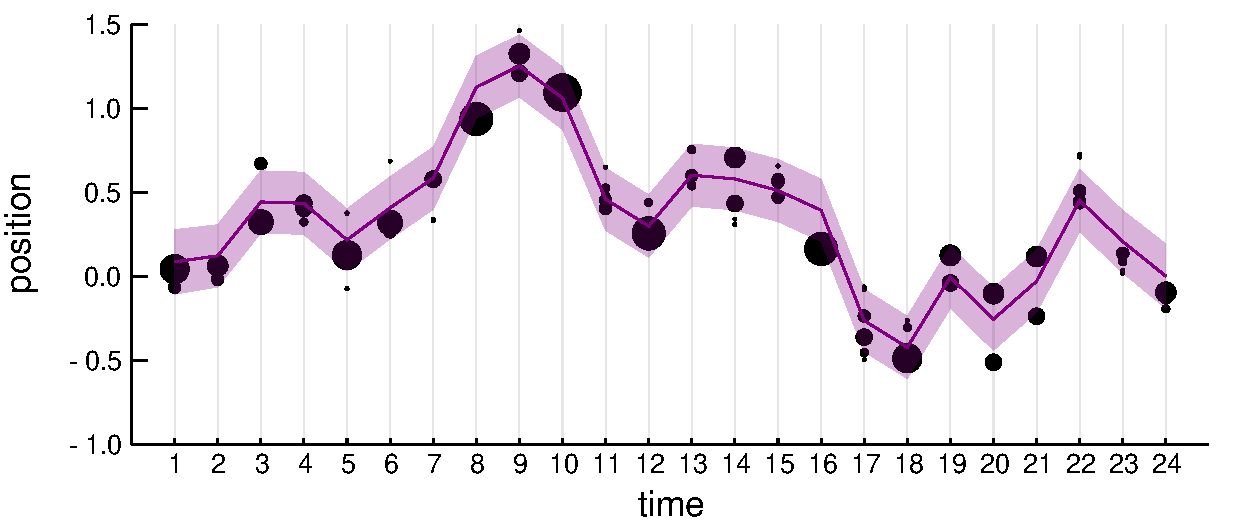
\includegraphics[width=\colwidth]{../smc_kalman_3.pdf}
\caption{Exact posterior (purple) and weighted SMC particles before resampling (black) for a linear Gaussian HMM.}
\end{figure}
\end{block}

\begin{block}{Ancestral Degeneracy}
For some applications, we want to approximate the \emph{joint} distribution over all parameters.
We can approximate this distribution by the ``trajectories'' of each of the $N$ particles.\\[16pt]

However, due to resampling these trajectories overlap, coalescing backwards in time. At some point all the trajectories coalesce, and we approximate that parameter's distribution with just one point!

\begin{figure} %%% remake this plot with a less weird realisation? %%%
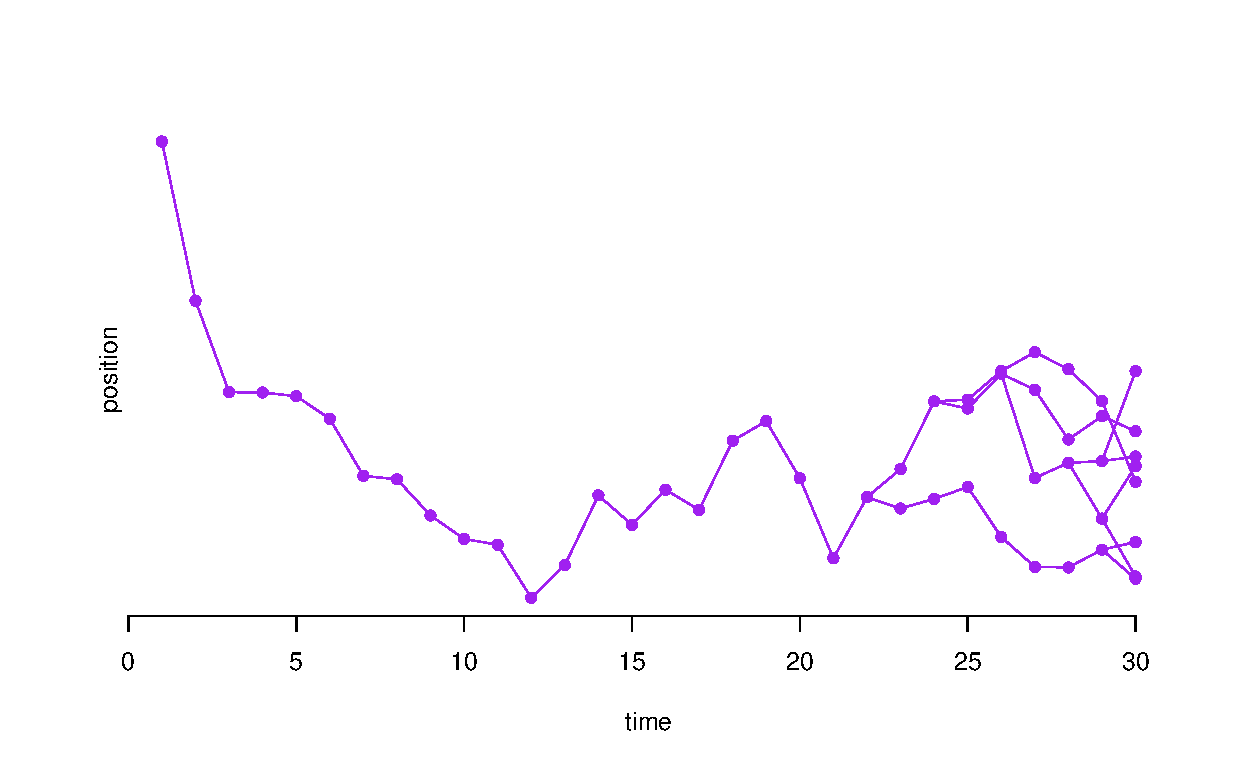
\includegraphics[width=\colwidth , trim={1.5cm 0.5cm 0.5cm 1.5cm},clip]{../degen2.pdf}
\caption{Trajectories from a sample of N=10 particles. At most points there are just one or two distinct samples.}
\end{figure}

This phenomenon is known as \emph{ancestral degeneracy}\textsuperscript{2}, since the joint structure of the trajectories can be viewed as a \emph{genealogy} of particles. It is one of the main issues with SMC, so we would like to analyse it.
\end{block}
\end{column}

\begin{column}{\colwidth}
\vspace*{5pt}

\begin{block}{The Kingman Coalescent\textsuperscript{3}}
\begin{columns}
\begin{column}{0.5\colwidth}
Kingman's $n$-coalescent is the coalescent process on a sample of $n$ individuals from a population of size $N$ in which each pair of lineages merges with unit rate.
It describes the limiting genealogies for a large class of population models when $N\to\infty$.
\end{column}
\begin{column}{0.5\colwidth}
\begin{center}
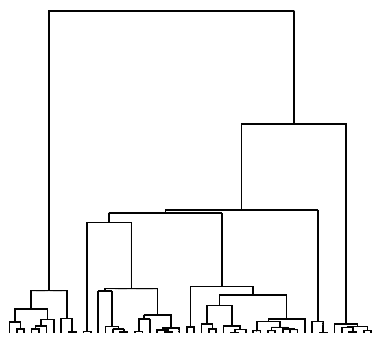
\includegraphics[width=0.7\textwidth]{../kingman.png}\\
\small{
\textbf{A realisation of the 50-coalescent.}
\textit{Source: Wikimedia Commons}
}
\end{center}
\end{column}
\end{columns}
\end{block}

\begin{block}{SMC Genealogies}
The genealogy depends on the number of offspring of each particle upon resampling at each time $t$, denoted $(\vt{1}, \dots, \vt{N})$.
A key quantity in the asymptotic analysis is the coalescence rate
\begin{equation*}
c_N(t) := \frac{1}{(N)_2} \sum_{i=1}^{N} \vt{i}(\vt{i}-1).
\end{equation*}

To obtain convergence to the Kingman coalescent, we rescale time by the inverse coalescence rate to achieve the required unit rate.\\[16pt]

It has been shown that, under such a rescaling and some standard assumptions, genealogies induced by multinomial resampling converge (in the sense of finite-dimensional distributions) to the Kingman coalescent\textsuperscript{4}. Simulations show the same structure even for finite $N$.\\[16pt]

We have since extended this result to cover conditional SMC\textsuperscript{5} with multinomial resampling. In this algorithm, a certain ``immortal trajectory'' is conditioned to survive all the resampling steps. This still admits the Kingman coalescent as its limiting genealogy, but simulations show different behaviour for $N<\infty$.\\[35pt]
\begin{figure}
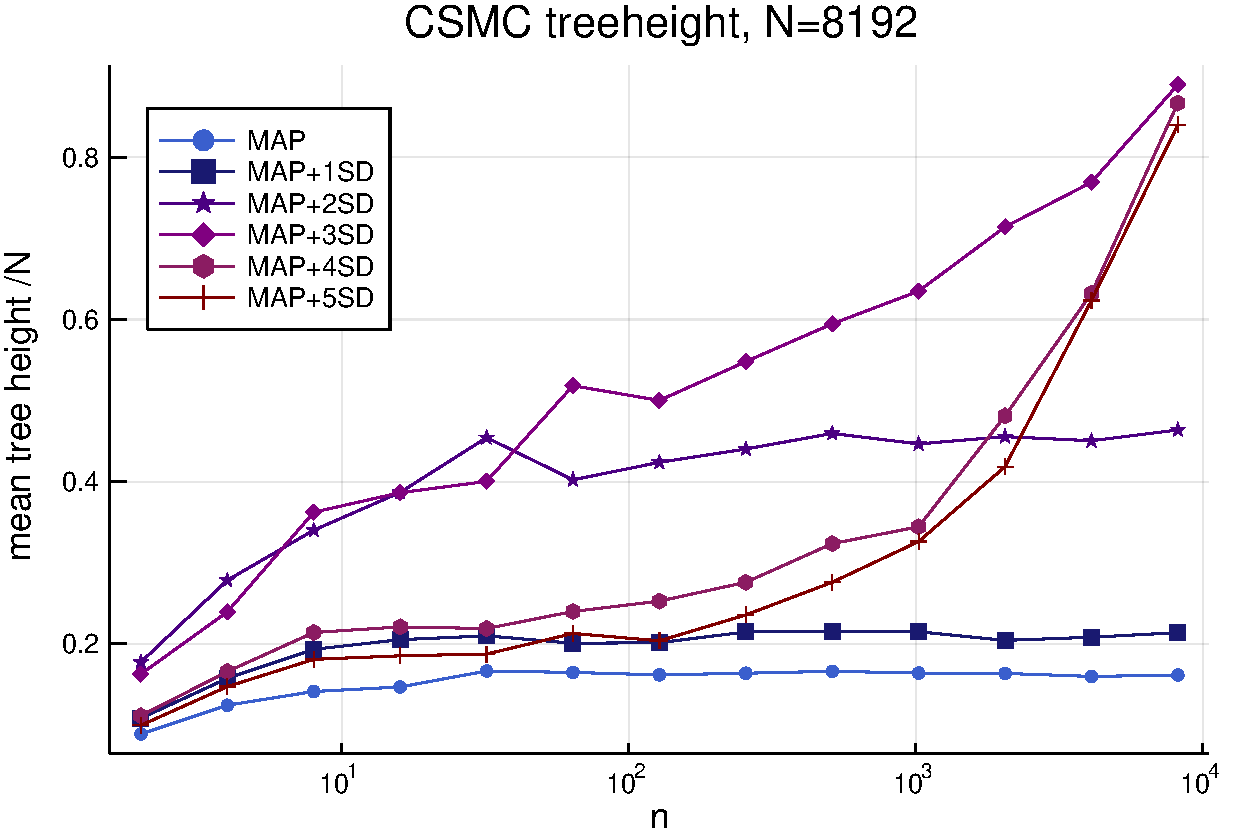
\includegraphics[width=\colwidth]{../CSMC_treeheight_500reps.pdf}
\caption{Average height of subtrees with $n$ randomly chosen nodes, for different choices of immortal trajectory.}
\end{figure}
We conjecture that the process undergoes a phase transition when the immortal trajectory is particularly ``unlikely'' and $n$ approaches $N$.
\end{block}

\vspace*{40pt}
\hrule
\begin{block}

\vspace*{-20pt}

\small{
\begin{enumerate}
\item Gordon, N. J., Salmond, D. J., \& Smith, A. F. (1993). Novel approach to nonlinear/non-Gaussian Bayesian state estimation. \textit{IEE:F} 140(3), 107-113.
\item Doucet, A., \& Johansen, A. M. (2011). A tutorial on particle filtering and smoothing: Fifteen years later. \textit{Handbook of nonlinear filtering}, 656-704. OUP.
\item Kingman, J.F.C. (1982). The coalescent. \textit{Stochastic processes and their applications}, 13(3), 235-248.
\item Koskela, J. et al. (2018).  Asymptotic genealogies of interacting particle systems with an application to sequential Monte Carlo. arXiv:1804.01811.
\item Andrieu, C., Doucet, A., \& Holenstein, R. (2010). Particle Markov chain Monte Carlo methods. \textit{RSS:B}, 72(3), 269-342.
\end{enumerate}
}
\end{block}

\end{column}
\end{columns}

\end{frame}
\end{document}